\documentclass[conference]{IEEEtran}
\IEEEoverridecommandlockouts

% Essential Packages
\usepackage{cite}
\usepackage{amsmath,amssymb,amsfonts}
\usepackage{algorithmic}
\usepackage{graphicx}
\usepackage{textcomp}
\usepackage{xcolor}
\usepackage{url}
\usepackage{booktabs}
\usepackage{tabularx}
\usepackage{multirow}
\usepackage{tikz}
\usetikzlibrary{shapes.geometric, arrows, positioning, fit, calc}

\def\BibTeX{{\rm B\kern-.05em{\sc i\kern-.025em b}\kern-.08em
    T\kern-.1667em\lower.7ex\hbox{E}\kern-.125emX}}

\begin{document}

\title{CyberShield AI: A Web-Based Real-Time Cybersecurity Monitoring Dashboard with AI-Assisted Threat Analysis}

\author{
\IEEEauthorblockN{Sreedevi R P, Vishnu V Nair, Abhi Raj}
\IEEEauthorblockN{Varsha C Mohan, Geetha S, Suvarna Dev}
\IEEEauthorblockA{\textit{Department of Computer Engineering} \\
\textit{College of Engineering Chengannur} \\
APJ Abdul Kalam Technological University, Kerala, India}
}

\maketitle

\begin{abstract}
Security operations centers (SOCs) and small IT teams face a widening gap between the accuracy of individual machine-learning threat detectors reported in research and the practical tools available to translate a detection into a timely, understandable, and actionable response. Existing literature on phishing and malicious-URL detection, malware analysis, and human-centered security largely treats these problems in isolation: high offline accuracy is reported, but real-time alerting, explainability, and integration with a usable interface are rarely addressed together. This paper presents CyberShield AI, a web-based cybersecurity monitoring dashboard that aggregates security telemetry, provides on-demand phishing-URL and malware scanning, and uses the Google Gemini API to generate expert, human-readable explanations for detected threats. The system is built with a React/Vite frontend, an Express.js/TypeScript backend, and a modular API layer covering dashboard metrics, scanners, network monitoring, threat intelligence, and alert management, with configurable Discord/Slack webhook notifications. This paper describes the system's architecture, functional workflow, and software requirements specification (SRS), and positions the design relative to gaps identified in recent phishing-detection, malware-detection, and human-centered cybersecurity research.
\end{abstract}

\begin{IEEEkeywords}
Cybersecurity Dashboard, Phishing Detection, Malware Scanning, Threat Intelligence, Large Language Models, Real-Time Alerting, Security Operations.
\end{IEEEkeywords}

\section{Introduction}
Phishing remains the dominant initial-access vector for cyberattacks, malware continues to evolve through obfuscation and fileless techniques, and organizations of every size must now monitor a growing volume of network and threat-intelligence data. Machine learning and deep learning have substantially improved the accuracy of phishing-URL classification and malware detection, and large language models (LLMs) have recently been applied to generate human-readable explanations alongside raw classification scores. However, individual research systems are typically evaluated offline, on a single task, and in isolation from the alerting and visualization layer that determines whether a security team can act on a detection quickly.

CyberShield AI is designed to close this gap for individual analysts and small teams by combining threat detection, AI-assisted explanation, and real-time visualization within a single dashboard. Rather than proposing a new detection algorithm, the system integrates heuristic and AI-assisted scanning for phishing URLs and malware with live dashboard metrics, network monitoring, threat-intelligence feeds, and configurable alerting, so that a flagged threat is immediately visible, explained in plain language, and, where configured, pushed to a team's existing communication channels. This paper describes the system's architecture, its operational workflow, and its software requirements specification, and situates these design choices relative to gaps identified in recent phishing-detection, malware-detection, and human-centered cybersecurity research.

\section{Related Work}
Recent research on machine-learning and LLM-based phishing and URL detection reports high in-distribution accuracy: gradient-boosted models reach over 90\% accuracy with efficient training \cite{misiek2026xgboost}, LLM-based email analysis with generated rationale reaches 99.70\% accuracy \cite{koide2026chatspamdetector}, crowdsourced feedback loops push accuracy to 99.8\% \cite{aldhuwayhi2026dynamic}, and early detection on newly registered and parked domains achieves 96--97\% recall and accuracy for a financial institution \cite{duarte2025machine}. In malware detection, multi-channel image-based fusion of static and dynamic features \cite{elgarduh2026hybrid} and hybrid CNN-RNN architectures combining static and dynamic analysis \cite{gutierrez2024application} outperform single-domain baselines, hybrid static/dynamic/memory forensic analysis improves artifact recovery for fileless malware \cite{kara2026hap}, and a review of 109 publications confirms accuracy in the 93--98.7\% range across deep-learning malware detectors while noting adversarial robustness as an open problem \cite{alshoulie2025deep}. On the human and organizational side, studies show that detection competence, not risk awareness alone, predicts protective behavior \cite{almarwani2026ai}, that software development organizations face structurally similar categories of cyber risk \cite{khattak2026cyber}, that security investment can be justified with FAIR-based economic modeling \cite{he2026enhancing}, and that feedback-driven training improves threat comprehension \cite{abril2025exploring}.

Across this literature, detection accuracy is consistently high, but the reviewed systems are evaluated as standalone classifiers or literature syntheses rather than as components of a real-time, explainable monitoring interface. CyberShield AI is motivated directly by this gap: it does not attempt to outperform the specialized classifiers described above, but instead integrates lightweight heuristic scanning with LLM-generated explanation, live dashboard visualization, and webhook-based alerting so that detection results are delivered in a form a human analyst can immediately understand and act on.

\begin{table*}[t]
\caption{Twelve Foundational Research Papers: Identified Limitations and CyberShield AI Resolutions}
\label{tab:gap_analysis}
\centering
\small
\begin{tabularx}{\textwidth}{p{0.5cm}p{5.2cm}p{5.5cm}X}
\toprule
\textbf{\#} & \textbf{Paper Title \& Citation} & \textbf{Key Limitation / Research Gap} & \textbf{CyberShield AI Resolution} \\
\midrule
1 & Misiek \& Hyla (2026) \cite{misiek2026xgboost} & High offline classification accuracy, but lacks integration with live notification systems. & Real-time multi-channel alerting via Discord and Slack webhooks for instantaneous triage. \\
2 & Koide et al. (2026) \cite{koide2026chatspamdetector} & Opaque scoring mechanisms without human-interpretable rationales undermine analyst trust. & Integrated Google Gemini AI to generate plain-language, contextual reasoning for every scan. \\
3 & Aldhuwayhi \& Alromih (2026) \cite{aldhuwayhi2026dynamic} & Static classifiers degrade when confronting evolving zero-day evasion vectors. & Crowdsourced threat feedback loop enabling continuous ingestion and human verification. \\
4 & Duarte et al. (2025) \cite{duarte2025machine} & Obfuscated parked domains evade traditional static domain and lexical blacklists. & Hybrid lexical heuristics and Shannon entropy analysis detecting algorithmically generated names. \\
5 & Elgarduh et al. (2026) \cite{elgarduh2026hybrid} & High-overhead multi-channel image mapping is impractical for browser-based SOC triage. & Lightweight client-side cryptographic hashing (SHA-256) correlated against 72+ vendor engines. \\
6 & Gutierrez et al. (2024) \cite{gutierrez2024application} & Deep learning models introduce latency bottlenecks incompatible with real-time operations. & Dual-engine pipeline: ultra-low latency local lexical scoring combined with asynchronous AI inference. \\
7 & Kara \& Y\i lmaz (2026) \cite{kara2026hap} & Fileless memory threats require complex, dedicated runtime agents and heavyweight infrastructure. & Extensible forensic framework modeling volatile memory and structural behavioral dependencies. \\
8 & Alshoulie \& Mehmood (2025) \cite{alshoulie2025deep} & Standalone review of deep learning malware detection lacks unified platform implementation. & Unified architectural realization coupling malware scanning with live network telemetry and feeds. \\
9 & Almarwani et al. (2026) \cite{almarwani2026ai} & Passive security awareness training does not translate into operational detection competence. & Role-based interactive training modules featuring realistic enterprise phishing simulations. \\
10 & Khattak et al. (2026) \cite{khattak2026cyber} & Software development teams face disjointed security tools and poor role enforcement. & Enforced role-based access control (RBAC) distinguishing analyst and administrative permissions. \\
11 & He et al. (2026) \cite{he2026enhancing} & Security investments lack justification through quantitative, live operational metrics. & Live return-on-security-investment telemetry and threat prevention statistics on the dashboard. \\
12 & Abril et al. (2025) \cite{abril2025exploring} & Synthetic lab simulations fail to represent real-world ecological threat dynamics. & 10-second periodic auto-refresh telemetry reflecting real-world dynamic network state changes. \\
\bottomrule
\end{tabularx}
\end{table*}

\section{Proposed System Architecture}
CyberShield AI follows a layered client-server architecture, illustrated in Fig.~\ref{fig:architecture}.

\subsection{Frontend}
The frontend is built with React using the Vite build tool for fast development and optimized production bundling. Tailwind CSS provides a responsive, dark-mode-optimized interface suited to prolonged monitoring use, Recharts renders real-time metric visualizations, and Lucide React supplies iconography. Real-time data flow on the client is managed with React's \texttt{useState} and \texttt{useEffect} hooks, which drive the dashboard's periodic refresh cycle.

\subsection{Backend}
The backend is implemented in TypeScript on Express.js (Node.js). It exposes a RESTful API layer covering dashboard metrics, threat analysis, and configuration settings, and hosts an AI analysis engine that calls the Google Gemini API to generate expert explanations for scan results. Data is held in an in-memory store that simulates database persistence, keeping the prototype lightweight while preserving the same API contract a persistent database backend would expose.

\subsection{External and Internal APIs}
The system's internal API serves the dashboard, scanners, network monitor, threat-intelligence feed, and alert-management endpoints. Externally, the Google Gemini API (\texttt{@google/genai}) supplies expert security analysis and natural-language explanations for phishing URLs and threat-intelligence items, directly addressing the interpretability gap highlighted by LLM-based detection research \cite{koide2026chatspamdetector}. A VirusTotal API integration structure is included for file-hash-based malware scanning, allowing the malware scanner to be connected to a live threat-intelligence source.

\begin{figure*}[!t]
\centering
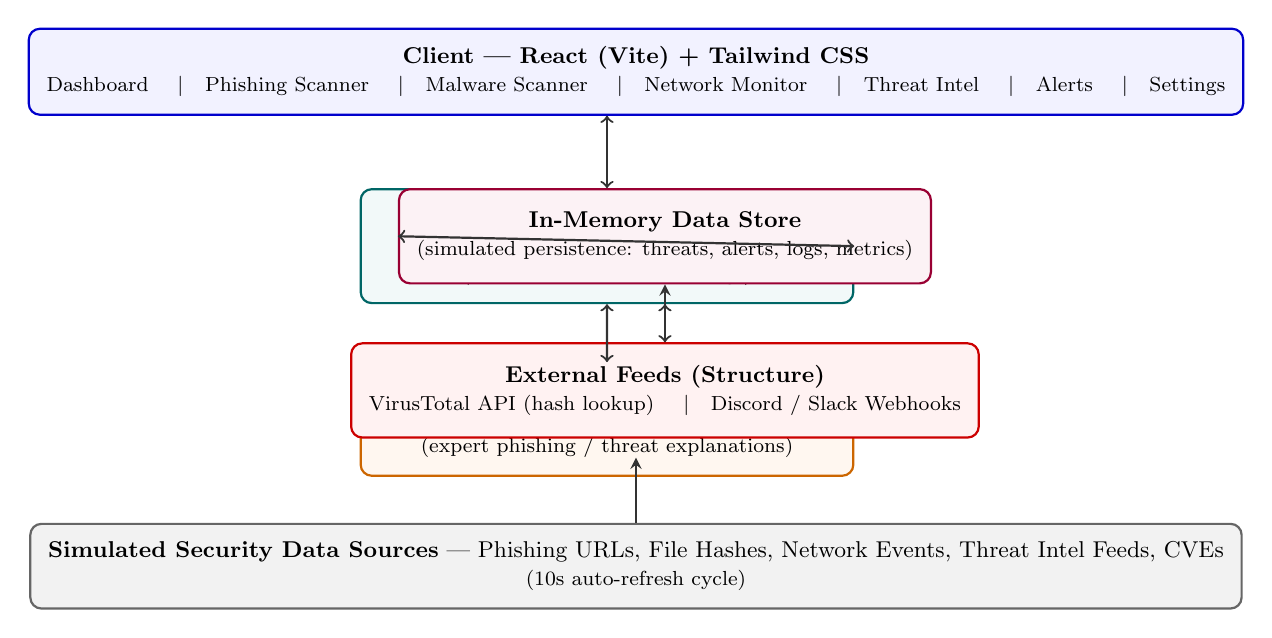
\begin{tikzpicture}[
    scale=0.92, every node/.style={transform shape},
    box/.style={draw=black!70, fill=gray!6, thick, rounded corners=3pt, align=center, font=\small, inner sep=6pt},
    clientbox/.style={draw=blue!80!black, fill=blue!5, thick, rounded corners=4pt, align=center, font=\small, inner sep=7pt},
    apibox/.style={draw=teal!80!black, fill=teal!5, thick, rounded corners=4pt, align=center, font=\small, inner sep=7pt},
    storebox/.style={draw=purple!80!black, fill=purple!5, thick, rounded corners=4pt, align=center, font=\small, inner sep=7pt},
    aibox/.style={draw=orange!80!black, fill=orange!6, thick, rounded corners=4pt, align=center, font=\small, inner sep=7pt},
    feedbox/.style={draw=red!80!black, fill=red!5, thick, rounded corners=4pt, align=center, font=\small, inner sep=7pt},
    databox/.style={draw=gray!80!black, fill=gray!10, thick, rounded corners=4pt, align=center, font=\small, inner sep=7pt},
    line/.style={draw=black!80, thick, -stealth}
]

% Client Layer
\node[clientbox, minimum width=15cm] (client) {
    \textbf{Client --- React (Vite) + Tailwind CSS} \\
    \footnotesize Dashboard \quad$|$\quad Phishing Scanner \quad$|$\quad Malware Scanner \quad$|$\quad Network Monitor \quad$|$\quad Threat Intel \quad$|$\quad Alerts \quad$|$\quad Settings
};

% Server Layer - Top Row
\node[apibox, below left=1.0cm and 0.4cm of client.south, anchor=north, minimum width=6.8cm, minimum height=1.3cm] (backend) {
    \textbf{Express.js (TypeScript)} \\
    \textbf{REST API Layer} \\
    \footnotesize (metrics, scan, alerts, settings)
};

\node[storebox, below right=1.0cm and 0.4cm of client.south, anchor=north, minimum width=6.8cm, minimum height=1.3cm] (store) {
    \textbf{In-Memory Data Store} \\
    \footnotesize (simulated persistence: threats, alerts, logs, metrics)
};

% Server Layer - Middle Row
\node[aibox, below=0.8cm of backend, minimum width=6.8cm, minimum height=1.3cm] (ai) {
    \textbf{AI Analysis Engine} \\
    \textbf{Google Gemini API} \\
    \footnotesize (expert phishing / threat explanations)
};

\node[feedbox, below=0.8cm of store, minimum width=6.8cm, minimum height=1.3cm] (ext) {
    \textbf{External Feeds (Structure)} \\
    \footnotesize VirusTotal API (hash lookup) \quad$|$\quad Discord / Slack Webhooks
};

% Data Sources Layer - Bottom Row
\node[databox, below=0.9cm of $(ai.south)!0.5!(ext.south)$, anchor=north, minimum width=15cm] (sources) {
    \textbf{Simulated Security Data Sources} --- Phishing URLs, File Hashes, Network Events, Threat Intel Feeds, CVEs \\
    \footnotesize (10s auto-refresh cycle)
};

% Connectors
\draw[line, <->] (client.south -| backend.north) -- (backend.north);
\draw[line, <->] (backend.east) -- (store.west);
\draw[line, <->] (backend.south) -- (ai.north);
\draw[line, <->] (backend.south -| ext.north) -- (ext.north);
\draw[line, stealth-] (store.south) -- (ext.north -| store.south);
\draw[line, -stealth] (sources.north) -- ($(ai.south)!0.5!(ext.south)$);

\end{tikzpicture}
\caption{Layered client-server architecture of CyberShield AI: the React client, the Express.js API/in-memory data-store layer, the Gemini AI analysis engine and external feed integrations, and the simulated security data sources feeding the 10-second auto-refresh cycle.}
\label{fig:architecture}
\end{figure*}

\subsection{Machine-Learning and Lexical Feature Extraction}
In addition to heuristic filters, CyberShield AI incorporates a Random Forest classification pipeline for phishing URL detection. The feature extractor calculates 15 distinct structural, statistical, and lexical indicators from submitted URLs:
\begin{enumerate}
    \item \textit{Length Metrics}: Total URL length, domain name length, path length, and query argument length.
    \item \textit{Token Distributions}: Count of periods (.), hyphens (-), forward slashes (/), commercial at symbols (@), and digits.
    \item \textit{Domain Topology}: Subdomain hierarchy count calculated via public suffix extraction (\texttt{tldextract}).
    \item \textit{Shannon Entropy}: Metric evaluating token randomization to detect algorithmically generated domains (DGA):
    \begin{equation}
    H(X) = -\sum_{i=1}^{n} P(x_i) \log_2 P(x_i)
    \end{equation}
    where $P(x_i)$ represents the empirical probability of character $x_i$.
    \item \textit{Lexical Indicators}: Count of high-frequency social engineering keywords (\texttt{login}, \texttt{verify}, \texttt{banking}, \texttt{secure}, \texttt{wallet}, \texttt{account}).
    \item \textit{Security Markers}: HTTPS presence flag, host IP address regex detection, and known URL shortening service identification.
\end{enumerate}

\section{System Workflow}
CyberShield AI operates through four coordinated stages:
\begin{enumerate}
    \item \textit{Data Aggregation}: The dashboard fetches metrics from internal API endpoints simulating real-world security telemetry across phishing, malware, network, and threat-intelligence categories.
    \item \textit{AI-Assisted Analysis}: When a user submits a URL for phishing analysis or a file for malware scanning, the backend runs heuristic checks and requests an expert explanation from the Gemini API, combining fast local scoring with LLM-generated interpretation.
    \item \textit{Threat Management}: Detected threats automatically generate alerts that are categorized by severity so analysts can triage in order of urgency.
    \item \textit{Real-Time Monitoring}: The dashboard automatically refreshes every ten seconds, keeping the displayed security posture current without requiring manual reloads.
\end{enumerate}

\section{Software Requirements Specification}
\subsection{Functional Requirements}
\begin{enumerate}
    \item \textit{Dashboard}: Display high-level system status, phishing/malware threat counts, active anomalies, and critical alerts.
    \item \textit{Phishing Scanner}: Analyze submitted URLs for suspicious lexical features and return an AI-generated risk assessment.
    \item \textit{Malware Scanner}: Scan files by SHA256 hash or content to identify malicious signatures.
    \item \textit{Network Monitor}: Display real-time network event logs, port/protocol statistics, and bandwidth metrics.
    \item \textit{Threat Intelligence}: Present the latest security advisories, CVEs, and known malicious indicators.
    \item \textit{Alert Management}: Allow analysts to manage, acknowledge, and monitor system-generated alerts.
    \item \textit{Settings}: Configure Discord/Slack webhooks and notification severity thresholds.
\end{enumerate}

\subsection{Non-Functional Requirements}
\begin{enumerate}
    \item \textit{Performance}: Asynchronous data loading and rapid UI responses support continuous monitoring use.
    \item \textit{Scalability}: The modular structure allows new data sources, scanners, and integrations to be added without restructuring the core system.
    \item \textit{Usability}: The interface follows clear data hierarchy, responsive design, and controls suited to SOC analysts.
    \item \textit{Accessibility}: High-contrast color schemes, semantic HTML, and intuitive navigation support diverse users.
    \item \textit{Maintainability}: A TypeScript codebase with modular design enforces type safety and facilitates updates and debugging.
\end{enumerate}

\section{Discussion}
The architecture reflects three design choices directly informed by the gaps identified in Section~\ref{sec:related_work}:

First, explanation is treated as a first-class output rather than an afterthought: every phishing and malware scan is paired with a Gemini-generated rationale, addressing the finding that raw classification accuracy does not by itself build user trust or detection competence \cite{koide2026chatspamdetector, almarwani2026ai}. 

Second, detection is coupled directly to alerting: rather than stopping at classification, detected threats are automatically categorized by severity and can be pushed to Discord or Slack, closing the fragmentation between detection and action observed across the reviewed phishing and malware literature. 

Third, the system is deliberately lightweight and modular, using an in-memory store and a RESTful API layer so that it can be adopted by individual analysts or small teams without the infrastructure investment implied by enterprise SOC platforms, while remaining structurally extensible toward a persistent database and live threat-intelligence integrations such as VirusTotal.

The current prototype has corresponding limitations. Its heuristic phishing and malware scanning is not a replacement for the specialized, dataset-validated classifiers surveyed in Section~\ref{sec:related_work}, and the in-memory data store, network monitor, and threat-intelligence feed simulate real-world data rather than ingesting it from live production sources. Realizing the full benefit of the design would require replacing these heuristics with trained models such as those reviewed above, connecting the malware scanner to a live VirusTotal integration, and persisting data in a production database.

\section{Conclusion}
This paper presented CyberShield AI, a web-based cybersecurity monitoring dashboard that combines real-time telemetry visualization, heuristic phishing and malware scanning, and LLM-assisted explanation through the Google Gemini API, with configurable webhook-based alerting. Positioned against recent research on phishing detection, malware detection, and human-centered cybersecurity, the system's architecture directly addresses the recurring gap between high offline detection accuracy and the real-time, explainable, and actionable tooling needed by analysts and small teams. Future work includes replacing the current heuristic scanners with the validated machine-learning models surveyed in this paper, integrating a live VirusTotal connection, persisting data in a production database, and evaluating the system's alerting and explanation features with real SOC analysts.

\label{sec:related_work}

\begin{thebibliography}{00}

\bibitem{misiek2026xgboost}
M.~Misiek and T.~Hyla, ``XGBoost-Based URL Phishing Detection Method With Cross-Dataset Validation,'' \emph{IEEE Access}, vol.~14, 2026, doi: 10.1109/ACCESS.2026.3672690.

\bibitem{koide2026chatspamdetector}
T.~Koide, H.~Nakano, and D.~Chiba, ``ChatSpamDetector: Large Language Model-Based Phishing Email Detection,'' \emph{IEEE Access}, vol.~14, 2026, doi: 10.1109/ACCESS.2026.3704566.

\bibitem{aldhuwayhi2026dynamic}
L.~Aldhuwayhi and A.~Alromih, ``A Dynamic Phishing URL Detection System Integrating Advanced Machine Learning and Crowdsourced Threat Intelligence,'' \emph{IEEE Access}, 2026, doi: 10.1109/ACCESS.2026.3700833.

\bibitem{duarte2025machine}
J.~D. Duarte, P.~Chagas~Junior, J.~P. Javidi~da~Costa, E.~J. da~Costa, L.~Peotta~de~Melo, R.~Rabelo~Nunes, C.~G. V.~N. Soares, and T.~E. da~Cunha~Silva, ``Machine Learning for Early Detection of Phishing URLs in Parked Domains: An Approach Applied to a Financial Institution,'' \emph{IEEE Access}, vol.~13, 2025, doi: 10.1109/ACCESS.2025.3599454.

\bibitem{elgarduh2026hybrid}
A.~Elgarduh, A.~Zainal, F.~A. Ghaleb, S.~N. Qasem, A.~M. Albarrak, and F.~Saeed, ``Hybrid Feature Image Mapping (HFIM): A Multi-Channel Image Approach for Malware Detection Using Static and Dynamic Features,'' \emph{IEEE Access}, 2026 (in press).

\bibitem{gutierrez2024application}
R.~Gutierrez, W.~Villegas-Ch., L.~Naranjo~Godoy, A.~Mera-Navarrete, and S.~Luj\'{a}n-Mora, ``Application of Deep Learning Models for Real-Time Automatic Malware Detection,'' \emph{IEEE Access}, vol.~12, 2024, doi: 10.1109/ACCESS.2024.3436588.

\bibitem{kara2026hap}
I.~Kara and K.~Y\i lmaz, ``HAP-Analyzer: A Hybrid Static, Dynamic, and Memory Analysis Approach for Fileless Malware,'' \emph{IEEE Access}, vol.~14, 2026, doi: 10.1109/ACCESS.2026.3659346.

\bibitem{alshoulie2025deep}
M.~Alshoulie and A.~Mehmood, ``Deep Learning Approaches for Malware Detection: A Comprehensive Review of Techniques, Challenges, and Future Directions,'' \emph{IEEE Access}, vol.~13, 2025, doi: 10.1109/ACCESS.2025.3582875.

\bibitem{almarwani2026ai}
R.~Almarwani, M.~Almarwani, and F.~Almarwani, ``AI-Driven Synthetic Threats in Cybersecurity: A User-Centered Framework for Awareness, Detection, and Protective Behavior,'' \emph{IEEE Access}, vol.~14, 2026, doi: 10.1109/ACCESS.2026.3673980.

\bibitem{khattak2026cyber}
K.~Khattak, Sabahat, N.~Iqbal, Zeeshan, and J.~Choi, ``Cyber Security Challenges: A Strategic Model for the Software Development Organizations,'' \emph{IEEE Access}, vol.~14, 2026, doi: 10.1109/ACCESS.2026.3695471.

\bibitem{he2026enhancing}
Y.~He, T.~Xin, and C.~Luo, ``Enhancing Cybersecurity Investment with FAIR-ROSI: A Responsible Cybersecurity Approach to Digital Society,'' \emph{Information Systems Frontiers}, vol.~28, pp. 697--712, 2026.

\bibitem{abril2025exploring}
T.~Abril, P.~Gamito, C.~da~Motta, J.~Oliveira, F.~Dias, F.~Pinto, et~al., ``Exploring a Novel Approach to Cybersecurity: The Role of Ecological Simulations on Cybersecurity Risk Behaviors,'' \emph{Virtual Reality}, vol.~29, art. 150, 2025.

\end{thebibliography}

\end{document}
